\documentclass[a4paper,11pt]{article}
\usepackage[margin=2cm]{geometry}

\usepackage[titletoc,toc,title,page]{appendix}
\usepackage[nodayofweek]{datetime}
\usepackage{cite}
\usepackage{graphicx}
\longdate

\usepackage{minted}
\usepackage{titlesec}
\usepackage{hyperref}
\usepackage{fancyhdr}
\pagestyle{fancyplain}
\fancyhf{}
\lhead{\fancyplain{}{M.Sc.\ Group Project Report}}
\rhead{\fancyplain{}{\today}}
\cfoot{\fancyplain{}{\thepage}}


\title{Implementation of attentional bistability of the dragonfly visual neurons in an intelligent biomimetic agent\\\Large{--- Final Report ---}}
\author{Juan Carlos Farah, Panagiotis Almpouras, Ioannis Kasidakis, Erik Grabljevec, Christos Kaplanis\\
       \{jcf214, pa512, ik311, eg1114, ck2714\}@doc.ic.ac.uk\\ \\
       \small{Supervisors: Professor Murray Shanahan, Zafeirios Fountas, Pedro Mediano}\\
       \small{Course: CO530/533, Imperial College London}
}

\begin{document}
\section{Action Selection}
\subsection{Methodology}
The function of this module is to convert the output of the pattern recognition neurons into an action for the dragonfly to take in order for it to pursue insects in its visual field.
The main aspects we needed to consider were:
\begin{enumerate}
	\item The simulation environment of the dragonfly
	\item The embodiment of the dragonfly
	\item The actions available to the dragonfly within its environment
	\item How to convert the output of the pattern recognition neurons into actions
\end{enumerate}
Since the purpose of this project is to provide a tool for studying dragonfly vision rather than prey capture, we decided that having a complicated 3D simulated environment for the dragonfly was unnecessary. Instead, we decided to use the original retina input as a basis for the 'environment' for the dragonfly, and simply add a red circle to the animation input that corresponds to the dragonfly's focal point. The focal point would be moved around within the 2D plane of the visual input by the action selection mechanism and the focal point being overlapping with a target in the visual field would represent the dragonfly having caught the target. The actions available to the dragonfly's focal point would be up, down, left and right within the visual field. Therefore, the output of the action selection module would be a video of the original animation with the position of the dragonfly's focal point superimposed to each frame. An example is shown in Figure 1.

\begin{figure}[hb]
\centering
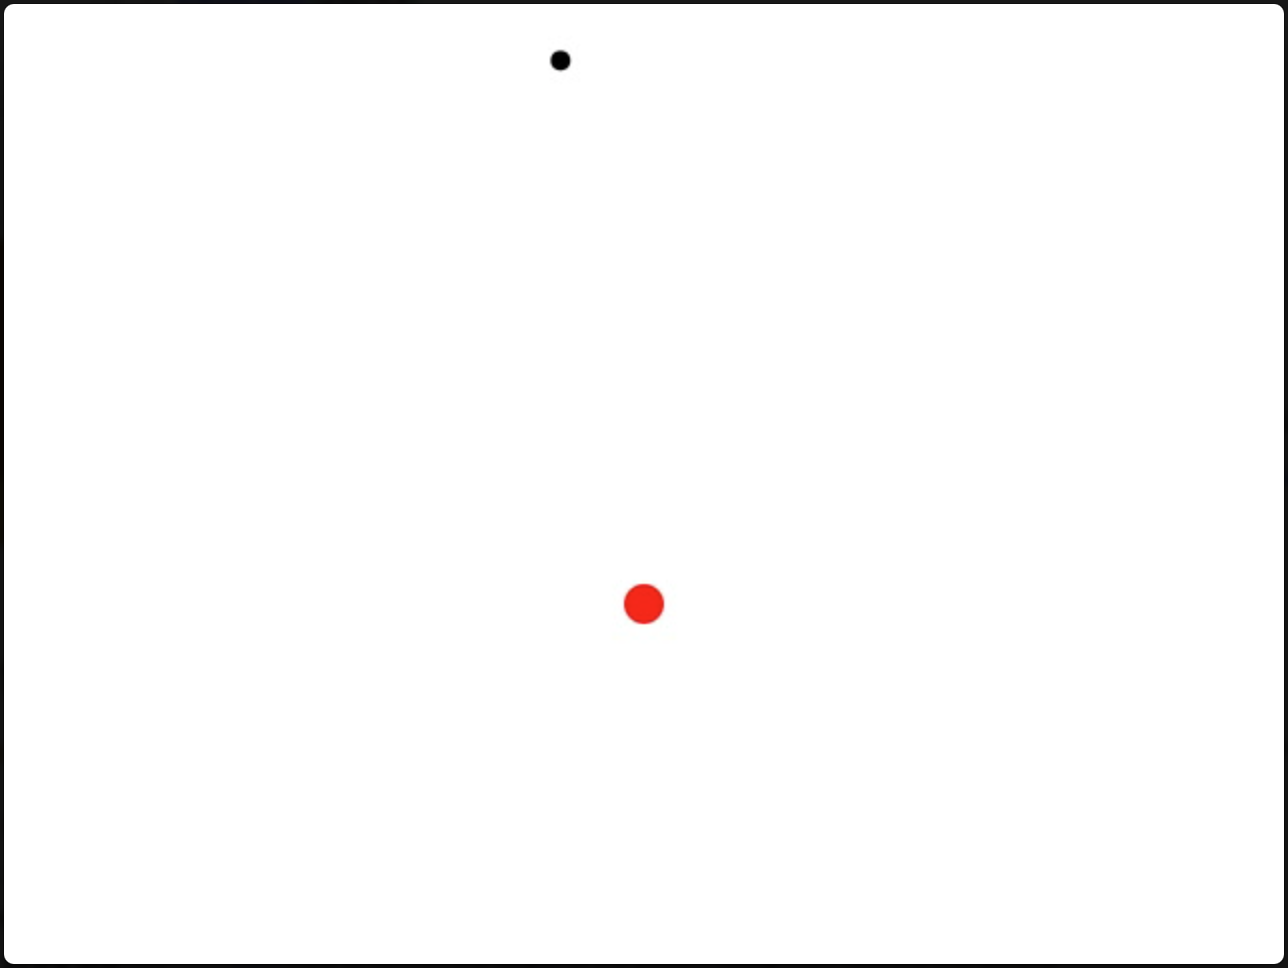
\includegraphics[scale = 0.3]{as_example}
\caption{Simple example of action selection output. The red dot represents the dragonfly focal point and the black dot represents the target.}
\end{figure}

In the original proposal for the project, it was suggested that we use reward-modulated reinforcement learning to train the action selection mechanism. The idea of this is to have a mechanism that can be used to train the dragonfly to choose the actions that maximize its reward, which is administered when it catches a target. 
\newline
\newline
We decided to implement a network of four action selection neurons, each representing one direction of movement (up, down, left and right). These neurons would take as input the spike train output of the pattern recognition neurons, via synapses with all-to-all connections between the two groups of neurons. The weights of the synapses would be initially randomised and the changes in weights would be dynamically governed by spike-timing-dependent plasticity (STDP, the same mechanism as the pattern recognition neurons) but modulated by a reward-modulator, which we label as dopamine but in reality could be another chemical. The way this works is that the change in weights determined by STDP is replaced with an eligibility trace that decays over time and the weights only change when dopamine is present in the system, by multiplying the eligibility trace of each synapse with the level of dopamine present. The dopamine is given a boost whenever the dragonfly focal point is within a certain distance of a target. The conceptual idea is that the synapses that contribute to catching the target are strengthened. The actual model used for the neurons is integrate-and-fire, which is a relatively simplistic but efficient model. The equations that govern the behaviour of the neurons and synapses are shown below: 
\newline
\newline
Integrate-and-fire neurons:
$$\frac{dv}{dt}=\frac{g _{e} (E_{e}-v _{r}) + E_{l} -v}{ \tau_{m}}$$
$$\frac{dg_{e}}{dt}= -\frac{g_{e}}{\tau_{e}}$$
where $v$ is the membrane potential, $g_{e}$ is the synaptic conductance, $E|{e}$ and $E_{l}$ are reverse potentials, $v_{r}$ is the resting potential and $\tau _{m}$ is a time constant.
\newline
Reward-modulated Synapses with STDP:
$$\frac{dw}{dt} = c \cdot Dop$$
$$\frac{dDop}{dt}=-\frac{Dop}{\tau _{Dop}}$$
$$\frac{dc}{dt} = -\frac{c}{\tau _{c}}$$
$$\frac{dApre}{dt}=-\frac{Apre}{\tau_{pre}}$$
$$\frac{dApost}{dt}=-\frac{Apost}{\tau_{post}}$$
where $w$ is the weight of the synapse, $c$ is the eligibility trace, $Dop$ is the level of dopamine, $dApre$ and $dApost$ are variables that govern the STDP and the $\tau$s are time constants.
When the pre-synaptic neuron fires, the following updates are executed:
$$ge = ge + w$$
$$Apre = Apre + Apre _{step}$$
$$c =c+Apost$$
When the post-synaptic neuron fires, the following updates are executed:
$$Apost = Apost + Apost _{step}$$
$$c =c+Apre$$
where $Apre_{step}$ and $Apost_{step}$ are constants.

Finally, at each time step, the distance between dragonfly's focal point (which is initialised to some position at the start) and the nearest target is calculated. If the distance is within a preset distance, a dopamine boost is administered to the system. The movement of the dragonfly is calculated by translating the firing rate of each of the four neurons into the velocity of the focal point in the corresponding direction. The overall velocity and hence distance travelled for the time step was averaged between the four and the dragonfly position updated. 

It is possible to run the action selection part in training mode, where the weights can change, or in fixed mode where you give it trained, fixed weights to simply run a simulation. 

The model was implemented in Python using a neuron simulator package called Brian 2 (CITATION). We used this as it is a flexible simulator and easier to use than NEURON (which was used for the CSTMD), since we are only modelling point neurons in this module, not a multi-compartmental model. 

The output of the action-selection module is twofold:
\begin{enumerate}
\item A video of the original animation with the dragonfly focal point position superimposed to each frame. This way you can see if the dragonfly is 'chasing' the targets or not.
\item A graphical display of the behaviour of variables of the model during the simulation, including weights, firing rates, the dopamine level and a raster plot.
\end{enumerate}
In the web client, the user is able to change the parameters of the model and observe how the resulting dragonfly's behaviour, as well as the behaviour of variables in the model.
\newline
\newline
Integrate-and-fire neurons:
$$\frac{dv}{dt}=\frac{g _{e} (E_{e}-v _{r}) + E_{l} -v}{ \tau_{m}}$$
$$\frac{dg_{e}}{dt}= -\frac{g_{e}}{\tau_{e}}$$
where $v$ is the membrane potential, $g_{e}$ is the synaptic conductance, $E_{e}$ and $E_{l}$ are reverse potentials, $v_{r}$ is the resting potential and $\tau _{m}$ is a time constant.
\newline
\newline
Reward-modulated synapses with STDP:
$$\frac{dw}{dt} = c \cdot Dop$$
$$\frac{dDop}{dt}=-\frac{Dop}{\tau _{Dop}}$$
$$\frac{dc}{dt} = -\frac{c}{\tau _{c}}$$
$$\frac{dApre}{dt}=-\frac{Apre}{\tau_{pre}}$$
$$\frac{dApost}{dt}=-\frac{Apost}{\tau_{post}}$$
where $w$ is the weight of the synapse, $c$ is the eligibility trace, $Dop$ is the level of dopamine, $dApre$ and $dApost$ are variables that govern the STDP, and the $\tau$s are time constants.
When the pre-synaptic neuron fires, the following updates are executed:
$$g_{e} = g_{e} + w$$
$$Apre = Apre + Apre _{step}$$
$$c =c+Apost$$
When the post-synaptic neuron fires, the following updates are executed, where $Apre_{step}$ and $Apost_{step}$ are constants.
$$Apost = Apost + Apost _{step}$$
$$c =c+Apre$$

\end{document}